
% Default to the notebook output style

    


% Inherit from the specified cell style.




    
\documentclass[11pt]{article}

    
    
    \usepackage[T1]{fontenc}
    % Nicer default font (+ math font) than Computer Modern for most use cases
    \usepackage{mathpazo}

    % Basic figure setup, for now with no caption control since it's done
    % automatically by Pandoc (which extracts ![](path) syntax from Markdown).
    \usepackage{graphicx}
    % We will generate all images so they have a width \maxwidth. This means
    % that they will get their normal width if they fit onto the page, but
    % are scaled down if they would overflow the margins.
    \makeatletter
    \def\maxwidth{\ifdim\Gin@nat@width>\linewidth\linewidth
    \else\Gin@nat@width\fi}
    \makeatother
    \let\Oldincludegraphics\includegraphics
    % Set max figure width to be 80% of text width, for now hardcoded.
    \renewcommand{\includegraphics}[1]{\Oldincludegraphics[width=.8\maxwidth]{#1}}
    % Ensure that by default, figures have no caption (until we provide a
    % proper Figure object with a Caption API and a way to capture that
    % in the conversion process - todo).
    \usepackage{caption}
    \DeclareCaptionLabelFormat{nolabel}{}
    \captionsetup{labelformat=nolabel}

    \usepackage{adjustbox} % Used to constrain images to a maximum size 
    \usepackage{xcolor} % Allow colors to be defined
    \usepackage{enumerate} % Needed for markdown enumerations to work
    \usepackage{geometry} % Used to adjust the document margins
    \usepackage{amsmath} % Equations
    \usepackage{amssymb} % Equations
    \usepackage{textcomp} % defines textquotesingle
    % Hack from http://tex.stackexchange.com/a/47451/13684:
    \AtBeginDocument{%
        \def\PYZsq{\textquotesingle}% Upright quotes in Pygmentized code
    }
    \usepackage{upquote} % Upright quotes for verbatim code
    \usepackage{eurosym} % defines \euro
    \usepackage[mathletters]{ucs} % Extended unicode (utf-8) support
    \usepackage[utf8x]{inputenc} % Allow utf-8 characters in the tex document
    \usepackage{fancyvrb} % verbatim replacement that allows latex
    \usepackage{grffile} % extends the file name processing of package graphics 
                         % to support a larger range 
    % The hyperref package gives us a pdf with properly built
    % internal navigation ('pdf bookmarks' for the table of contents,
    % internal cross-reference links, web links for URLs, etc.)
    \usepackage{hyperref}
    \usepackage{longtable} % longtable support required by pandoc >1.10
    \usepackage{booktabs}  % table support for pandoc > 1.12.2
    \usepackage[inline]{enumitem} % IRkernel/repr support (it uses the enumerate* environment)
    \usepackage[normalem]{ulem} % ulem is needed to support strikethroughs (\sout)
                                % normalem makes italics be italics, not underlines
    

    
    
    % Colors for the hyperref package
    \definecolor{urlcolor}{rgb}{0,.145,.698}
    \definecolor{linkcolor}{rgb}{.71,0.21,0.01}
    \definecolor{citecolor}{rgb}{.12,.54,.11}

    % ANSI colors
    \definecolor{ansi-black}{HTML}{3E424D}
    \definecolor{ansi-black-intense}{HTML}{282C36}
    \definecolor{ansi-red}{HTML}{E75C58}
    \definecolor{ansi-red-intense}{HTML}{B22B31}
    \definecolor{ansi-green}{HTML}{00A250}
    \definecolor{ansi-green-intense}{HTML}{007427}
    \definecolor{ansi-yellow}{HTML}{DDB62B}
    \definecolor{ansi-yellow-intense}{HTML}{B27D12}
    \definecolor{ansi-blue}{HTML}{208FFB}
    \definecolor{ansi-blue-intense}{HTML}{0065CA}
    \definecolor{ansi-magenta}{HTML}{D160C4}
    \definecolor{ansi-magenta-intense}{HTML}{A03196}
    \definecolor{ansi-cyan}{HTML}{60C6C8}
    \definecolor{ansi-cyan-intense}{HTML}{258F8F}
    \definecolor{ansi-white}{HTML}{C5C1B4}
    \definecolor{ansi-white-intense}{HTML}{A1A6B2}

    % commands and environments needed by pandoc snippets
    % extracted from the output of `pandoc -s`
    \providecommand{\tightlist}{%
      \setlength{\itemsep}{0pt}\setlength{\parskip}{0pt}}
    \DefineVerbatimEnvironment{Highlighting}{Verbatim}{commandchars=\\\{\}}
    % Add ',fontsize=\small' for more characters per line
    \newenvironment{Shaded}{}{}
    \newcommand{\KeywordTok}[1]{\textcolor[rgb]{0.00,0.44,0.13}{\textbf{{#1}}}}
    \newcommand{\DataTypeTok}[1]{\textcolor[rgb]{0.56,0.13,0.00}{{#1}}}
    \newcommand{\DecValTok}[1]{\textcolor[rgb]{0.25,0.63,0.44}{{#1}}}
    \newcommand{\BaseNTok}[1]{\textcolor[rgb]{0.25,0.63,0.44}{{#1}}}
    \newcommand{\FloatTok}[1]{\textcolor[rgb]{0.25,0.63,0.44}{{#1}}}
    \newcommand{\CharTok}[1]{\textcolor[rgb]{0.25,0.44,0.63}{{#1}}}
    \newcommand{\StringTok}[1]{\textcolor[rgb]{0.25,0.44,0.63}{{#1}}}
    \newcommand{\CommentTok}[1]{\textcolor[rgb]{0.38,0.63,0.69}{\textit{{#1}}}}
    \newcommand{\OtherTok}[1]{\textcolor[rgb]{0.00,0.44,0.13}{{#1}}}
    \newcommand{\AlertTok}[1]{\textcolor[rgb]{1.00,0.00,0.00}{\textbf{{#1}}}}
    \newcommand{\FunctionTok}[1]{\textcolor[rgb]{0.02,0.16,0.49}{{#1}}}
    \newcommand{\RegionMarkerTok}[1]{{#1}}
    \newcommand{\ErrorTok}[1]{\textcolor[rgb]{1.00,0.00,0.00}{\textbf{{#1}}}}
    \newcommand{\NormalTok}[1]{{#1}}
    
    % Additional commands for more recent versions of Pandoc
    \newcommand{\ConstantTok}[1]{\textcolor[rgb]{0.53,0.00,0.00}{{#1}}}
    \newcommand{\SpecialCharTok}[1]{\textcolor[rgb]{0.25,0.44,0.63}{{#1}}}
    \newcommand{\VerbatimStringTok}[1]{\textcolor[rgb]{0.25,0.44,0.63}{{#1}}}
    \newcommand{\SpecialStringTok}[1]{\textcolor[rgb]{0.73,0.40,0.53}{{#1}}}
    \newcommand{\ImportTok}[1]{{#1}}
    \newcommand{\DocumentationTok}[1]{\textcolor[rgb]{0.73,0.13,0.13}{\textit{{#1}}}}
    \newcommand{\AnnotationTok}[1]{\textcolor[rgb]{0.38,0.63,0.69}{\textbf{\textit{{#1}}}}}
    \newcommand{\CommentVarTok}[1]{\textcolor[rgb]{0.38,0.63,0.69}{\textbf{\textit{{#1}}}}}
    \newcommand{\VariableTok}[1]{\textcolor[rgb]{0.10,0.09,0.49}{{#1}}}
    \newcommand{\ControlFlowTok}[1]{\textcolor[rgb]{0.00,0.44,0.13}{\textbf{{#1}}}}
    \newcommand{\OperatorTok}[1]{\textcolor[rgb]{0.40,0.40,0.40}{{#1}}}
    \newcommand{\BuiltInTok}[1]{{#1}}
    \newcommand{\ExtensionTok}[1]{{#1}}
    \newcommand{\PreprocessorTok}[1]{\textcolor[rgb]{0.74,0.48,0.00}{{#1}}}
    \newcommand{\AttributeTok}[1]{\textcolor[rgb]{0.49,0.56,0.16}{{#1}}}
    \newcommand{\InformationTok}[1]{\textcolor[rgb]{0.38,0.63,0.69}{\textbf{\textit{{#1}}}}}
    \newcommand{\WarningTok}[1]{\textcolor[rgb]{0.38,0.63,0.69}{\textbf{\textit{{#1}}}}}
    
    
    % Define a nice break command that doesn't care if a line doesn't already
    % exist.
    \def\br{\hspace*{\fill} \\* }
    % Math Jax compatability definitions
    \def\gt{>}
    \def\lt{<}
    % Document parameters
    \title{01\_???????}
    
    
    

    % Pygments definitions
    
\makeatletter
\def\PY@reset{\let\PY@it=\relax \let\PY@bf=\relax%
    \let\PY@ul=\relax \let\PY@tc=\relax%
    \let\PY@bc=\relax \let\PY@ff=\relax}
\def\PY@tok#1{\csname PY@tok@#1\endcsname}
\def\PY@toks#1+{\ifx\relax#1\empty\else%
    \PY@tok{#1}\expandafter\PY@toks\fi}
\def\PY@do#1{\PY@bc{\PY@tc{\PY@ul{%
    \PY@it{\PY@bf{\PY@ff{#1}}}}}}}
\def\PY#1#2{\PY@reset\PY@toks#1+\relax+\PY@do{#2}}

\expandafter\def\csname PY@tok@gd\endcsname{\def\PY@tc##1{\textcolor[rgb]{0.63,0.00,0.00}{##1}}}
\expandafter\def\csname PY@tok@gu\endcsname{\let\PY@bf=\textbf\def\PY@tc##1{\textcolor[rgb]{0.50,0.00,0.50}{##1}}}
\expandafter\def\csname PY@tok@gt\endcsname{\def\PY@tc##1{\textcolor[rgb]{0.00,0.27,0.87}{##1}}}
\expandafter\def\csname PY@tok@gs\endcsname{\let\PY@bf=\textbf}
\expandafter\def\csname PY@tok@gr\endcsname{\def\PY@tc##1{\textcolor[rgb]{1.00,0.00,0.00}{##1}}}
\expandafter\def\csname PY@tok@cm\endcsname{\let\PY@it=\textit\def\PY@tc##1{\textcolor[rgb]{0.25,0.50,0.50}{##1}}}
\expandafter\def\csname PY@tok@vg\endcsname{\def\PY@tc##1{\textcolor[rgb]{0.10,0.09,0.49}{##1}}}
\expandafter\def\csname PY@tok@vi\endcsname{\def\PY@tc##1{\textcolor[rgb]{0.10,0.09,0.49}{##1}}}
\expandafter\def\csname PY@tok@vm\endcsname{\def\PY@tc##1{\textcolor[rgb]{0.10,0.09,0.49}{##1}}}
\expandafter\def\csname PY@tok@mh\endcsname{\def\PY@tc##1{\textcolor[rgb]{0.40,0.40,0.40}{##1}}}
\expandafter\def\csname PY@tok@cs\endcsname{\let\PY@it=\textit\def\PY@tc##1{\textcolor[rgb]{0.25,0.50,0.50}{##1}}}
\expandafter\def\csname PY@tok@ge\endcsname{\let\PY@it=\textit}
\expandafter\def\csname PY@tok@vc\endcsname{\def\PY@tc##1{\textcolor[rgb]{0.10,0.09,0.49}{##1}}}
\expandafter\def\csname PY@tok@il\endcsname{\def\PY@tc##1{\textcolor[rgb]{0.40,0.40,0.40}{##1}}}
\expandafter\def\csname PY@tok@go\endcsname{\def\PY@tc##1{\textcolor[rgb]{0.53,0.53,0.53}{##1}}}
\expandafter\def\csname PY@tok@cp\endcsname{\def\PY@tc##1{\textcolor[rgb]{0.74,0.48,0.00}{##1}}}
\expandafter\def\csname PY@tok@gi\endcsname{\def\PY@tc##1{\textcolor[rgb]{0.00,0.63,0.00}{##1}}}
\expandafter\def\csname PY@tok@gh\endcsname{\let\PY@bf=\textbf\def\PY@tc##1{\textcolor[rgb]{0.00,0.00,0.50}{##1}}}
\expandafter\def\csname PY@tok@ni\endcsname{\let\PY@bf=\textbf\def\PY@tc##1{\textcolor[rgb]{0.60,0.60,0.60}{##1}}}
\expandafter\def\csname PY@tok@nl\endcsname{\def\PY@tc##1{\textcolor[rgb]{0.63,0.63,0.00}{##1}}}
\expandafter\def\csname PY@tok@nn\endcsname{\let\PY@bf=\textbf\def\PY@tc##1{\textcolor[rgb]{0.00,0.00,1.00}{##1}}}
\expandafter\def\csname PY@tok@no\endcsname{\def\PY@tc##1{\textcolor[rgb]{0.53,0.00,0.00}{##1}}}
\expandafter\def\csname PY@tok@na\endcsname{\def\PY@tc##1{\textcolor[rgb]{0.49,0.56,0.16}{##1}}}
\expandafter\def\csname PY@tok@nb\endcsname{\def\PY@tc##1{\textcolor[rgb]{0.00,0.50,0.00}{##1}}}
\expandafter\def\csname PY@tok@nc\endcsname{\let\PY@bf=\textbf\def\PY@tc##1{\textcolor[rgb]{0.00,0.00,1.00}{##1}}}
\expandafter\def\csname PY@tok@nd\endcsname{\def\PY@tc##1{\textcolor[rgb]{0.67,0.13,1.00}{##1}}}
\expandafter\def\csname PY@tok@ne\endcsname{\let\PY@bf=\textbf\def\PY@tc##1{\textcolor[rgb]{0.82,0.25,0.23}{##1}}}
\expandafter\def\csname PY@tok@nf\endcsname{\def\PY@tc##1{\textcolor[rgb]{0.00,0.00,1.00}{##1}}}
\expandafter\def\csname PY@tok@si\endcsname{\let\PY@bf=\textbf\def\PY@tc##1{\textcolor[rgb]{0.73,0.40,0.53}{##1}}}
\expandafter\def\csname PY@tok@s2\endcsname{\def\PY@tc##1{\textcolor[rgb]{0.73,0.13,0.13}{##1}}}
\expandafter\def\csname PY@tok@nt\endcsname{\let\PY@bf=\textbf\def\PY@tc##1{\textcolor[rgb]{0.00,0.50,0.00}{##1}}}
\expandafter\def\csname PY@tok@nv\endcsname{\def\PY@tc##1{\textcolor[rgb]{0.10,0.09,0.49}{##1}}}
\expandafter\def\csname PY@tok@s1\endcsname{\def\PY@tc##1{\textcolor[rgb]{0.73,0.13,0.13}{##1}}}
\expandafter\def\csname PY@tok@dl\endcsname{\def\PY@tc##1{\textcolor[rgb]{0.73,0.13,0.13}{##1}}}
\expandafter\def\csname PY@tok@ch\endcsname{\let\PY@it=\textit\def\PY@tc##1{\textcolor[rgb]{0.25,0.50,0.50}{##1}}}
\expandafter\def\csname PY@tok@m\endcsname{\def\PY@tc##1{\textcolor[rgb]{0.40,0.40,0.40}{##1}}}
\expandafter\def\csname PY@tok@gp\endcsname{\let\PY@bf=\textbf\def\PY@tc##1{\textcolor[rgb]{0.00,0.00,0.50}{##1}}}
\expandafter\def\csname PY@tok@sh\endcsname{\def\PY@tc##1{\textcolor[rgb]{0.73,0.13,0.13}{##1}}}
\expandafter\def\csname PY@tok@ow\endcsname{\let\PY@bf=\textbf\def\PY@tc##1{\textcolor[rgb]{0.67,0.13,1.00}{##1}}}
\expandafter\def\csname PY@tok@sx\endcsname{\def\PY@tc##1{\textcolor[rgb]{0.00,0.50,0.00}{##1}}}
\expandafter\def\csname PY@tok@bp\endcsname{\def\PY@tc##1{\textcolor[rgb]{0.00,0.50,0.00}{##1}}}
\expandafter\def\csname PY@tok@c1\endcsname{\let\PY@it=\textit\def\PY@tc##1{\textcolor[rgb]{0.25,0.50,0.50}{##1}}}
\expandafter\def\csname PY@tok@fm\endcsname{\def\PY@tc##1{\textcolor[rgb]{0.00,0.00,1.00}{##1}}}
\expandafter\def\csname PY@tok@o\endcsname{\def\PY@tc##1{\textcolor[rgb]{0.40,0.40,0.40}{##1}}}
\expandafter\def\csname PY@tok@kc\endcsname{\let\PY@bf=\textbf\def\PY@tc##1{\textcolor[rgb]{0.00,0.50,0.00}{##1}}}
\expandafter\def\csname PY@tok@c\endcsname{\let\PY@it=\textit\def\PY@tc##1{\textcolor[rgb]{0.25,0.50,0.50}{##1}}}
\expandafter\def\csname PY@tok@mf\endcsname{\def\PY@tc##1{\textcolor[rgb]{0.40,0.40,0.40}{##1}}}
\expandafter\def\csname PY@tok@err\endcsname{\def\PY@bc##1{\setlength{\fboxsep}{0pt}\fcolorbox[rgb]{1.00,0.00,0.00}{1,1,1}{\strut ##1}}}
\expandafter\def\csname PY@tok@mb\endcsname{\def\PY@tc##1{\textcolor[rgb]{0.40,0.40,0.40}{##1}}}
\expandafter\def\csname PY@tok@ss\endcsname{\def\PY@tc##1{\textcolor[rgb]{0.10,0.09,0.49}{##1}}}
\expandafter\def\csname PY@tok@sr\endcsname{\def\PY@tc##1{\textcolor[rgb]{0.73,0.40,0.53}{##1}}}
\expandafter\def\csname PY@tok@mo\endcsname{\def\PY@tc##1{\textcolor[rgb]{0.40,0.40,0.40}{##1}}}
\expandafter\def\csname PY@tok@kd\endcsname{\let\PY@bf=\textbf\def\PY@tc##1{\textcolor[rgb]{0.00,0.50,0.00}{##1}}}
\expandafter\def\csname PY@tok@mi\endcsname{\def\PY@tc##1{\textcolor[rgb]{0.40,0.40,0.40}{##1}}}
\expandafter\def\csname PY@tok@kn\endcsname{\let\PY@bf=\textbf\def\PY@tc##1{\textcolor[rgb]{0.00,0.50,0.00}{##1}}}
\expandafter\def\csname PY@tok@cpf\endcsname{\let\PY@it=\textit\def\PY@tc##1{\textcolor[rgb]{0.25,0.50,0.50}{##1}}}
\expandafter\def\csname PY@tok@kr\endcsname{\let\PY@bf=\textbf\def\PY@tc##1{\textcolor[rgb]{0.00,0.50,0.00}{##1}}}
\expandafter\def\csname PY@tok@s\endcsname{\def\PY@tc##1{\textcolor[rgb]{0.73,0.13,0.13}{##1}}}
\expandafter\def\csname PY@tok@kp\endcsname{\def\PY@tc##1{\textcolor[rgb]{0.00,0.50,0.00}{##1}}}
\expandafter\def\csname PY@tok@w\endcsname{\def\PY@tc##1{\textcolor[rgb]{0.73,0.73,0.73}{##1}}}
\expandafter\def\csname PY@tok@kt\endcsname{\def\PY@tc##1{\textcolor[rgb]{0.69,0.00,0.25}{##1}}}
\expandafter\def\csname PY@tok@sc\endcsname{\def\PY@tc##1{\textcolor[rgb]{0.73,0.13,0.13}{##1}}}
\expandafter\def\csname PY@tok@sb\endcsname{\def\PY@tc##1{\textcolor[rgb]{0.73,0.13,0.13}{##1}}}
\expandafter\def\csname PY@tok@sa\endcsname{\def\PY@tc##1{\textcolor[rgb]{0.73,0.13,0.13}{##1}}}
\expandafter\def\csname PY@tok@k\endcsname{\let\PY@bf=\textbf\def\PY@tc##1{\textcolor[rgb]{0.00,0.50,0.00}{##1}}}
\expandafter\def\csname PY@tok@se\endcsname{\let\PY@bf=\textbf\def\PY@tc##1{\textcolor[rgb]{0.73,0.40,0.13}{##1}}}
\expandafter\def\csname PY@tok@sd\endcsname{\let\PY@it=\textit\def\PY@tc##1{\textcolor[rgb]{0.73,0.13,0.13}{##1}}}

\def\PYZbs{\char`\\}
\def\PYZus{\char`\_}
\def\PYZob{\char`\{}
\def\PYZcb{\char`\}}
\def\PYZca{\char`\^}
\def\PYZam{\char`\&}
\def\PYZlt{\char`\<}
\def\PYZgt{\char`\>}
\def\PYZsh{\char`\#}
\def\PYZpc{\char`\%}
\def\PYZdl{\char`\$}
\def\PYZhy{\char`\-}
\def\PYZsq{\char`\'}
\def\PYZdq{\char`\"}
\def\PYZti{\char`\~}
% for compatibility with earlier versions
\def\PYZat{@}
\def\PYZlb{[}
\def\PYZrb{]}
\makeatother


    % Exact colors from NB
    \definecolor{incolor}{rgb}{0.0, 0.0, 0.5}
    \definecolor{outcolor}{rgb}{0.545, 0.0, 0.0}



    
    % Prevent overflowing lines due to hard-to-break entities
    \sloppy 
    % Setup hyperref package
    \hypersetup{
      breaklinks=true,  % so long urls are correctly broken across lines
      colorlinks=true,
      urlcolor=urlcolor,
      linkcolor=linkcolor,
      citecolor=citecolor,
      }
    % Slightly bigger margins than the latex defaults
    
    \geometry{verbose,tmargin=1in,bmargin=1in,lmargin=1in,rmargin=1in}
    
    

    \begin{document}
    
    
    \maketitle
    
    

    
    \section{磁気モーメント}\label{ux78c1ux6c17ux30e2ux30fcux30e1ux30f3ux30c8}

\begin{itemize}
\item
  磁性における最も基本的な対象は、\texttt{磁気モーメント}である
\item
  古典電磁気学では\texttt{磁気モーメント}を\texttt{環状電流}と等価とみる
\item
  面積\(|d{\bf S}|\)の環状素片(\texttt{素}:大きさ無限小)に電流\({\bf I}\)が流れる時、\texttt{磁気モーメント}\(d{\bf \mu}\)は以下の式で表される(単位:\(Am^2\))

  \begin{itemize}
  \item
    ベクトル\(d{\bf S}\)の大きさ:ループの面積
  \item
    ベクトル\(d{\bf S}\)の方向:ループに垂直
  \end{itemize}
\end{itemize}

\begin{eqnarray}
d{\bf \mu}=Id{\bf S}
\end{eqnarray}

\begin{itemize}
\item
  これは、\texttt{磁気双極子}と等価である

  \begin{itemize}
  \item
    \texttt{磁気双極子}は\texttt{電気双極子}(間隔微笑の正負の電荷)と一見類似の振る舞いをするので、そう呼ばれる
  \item
    すなわち、\texttt{磁気モーメント}は「反対の磁化を持つ2つの磁気単極子が、ベクトル\(d{\bf S}\)と同方向に微小間隔で結ばれたもの」
  \end{itemize}
\end{itemize}

\begin{figure}
\centering
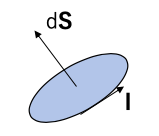
\includegraphics{./images/素環状電流による素磁気モーメント.png}
\caption{素環状電流による素磁気モーメント}
\end{figure}

    \begin{itemize}
\item
  磁気モーメント\(d{\bf \mu}\)は\textbf{環状電流の面に垂直}であり、ループを巡る電荷が担う\texttt{角運動量ベクトル}に\textbf{平行}または\textbf{反平行}である
\item
  大きさが有限のループが持つ磁気モーメント\(d{\bf \mu}\)を計算するには、

  \begin{itemize}
  \item
    そのループを等価な微小ループに分割し、
  \item
    微小環状電流が作る磁気モーメントを足し合わせれば良い
  \item
    隣接する微小ループの電流は全て相殺し、外周を流れる電流だけが残る
  \end{itemize}
\end{itemize}

\begin{eqnarray}
\bf \mu =\int d{\bf \mu} = I \int d{\bf S}
\end{eqnarray}

\begin{itemize}
\tightlist
\item
  多数の微小環状電流が作る磁気モーメントの和と見なされる
\end{itemize}

\begin{figure}
\centering
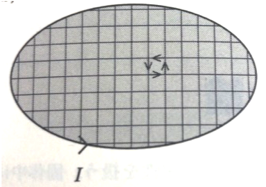
\includegraphics{./images/環状電流の和.png}
\caption{環状電流の和}
\end{figure}

    \subsection{1.
磁気モーメントと角運動量}\label{ux78c1ux6c17ux30e2ux30fcux30e1ux30f3ux30c8ux3068ux89d2ux904bux52d5ux91cf}

\begin{itemize}
\item
  \texttt{環状電流}は1つまたは複数の電荷の運動によるものである

  \begin{itemize}
  \item
    ここで考える電荷は全て質量を持つ粒子が担っている
  \item
    そのため、電荷はもちろん質量の軌道運動も存在し、磁気モーメントは常に角運動量と結びついている
  \end{itemize}
\item
  \texttt{原子}では、周回する電子が担う\texttt{磁気モーメント}\(d{\bf \mu}\)は、電子の角運動量\(d{\bf L}\)と同方向で、かつ\texttt{角運動量}に比例する

  \begin{itemize}
  \tightlist
  \item
    \(\gamma\):\texttt{磁気回転比}と呼ばれる定数
  \end{itemize}
\end{itemize}

\begin{eqnarray}
\bf \mu =\gamma{\bf L}
\end{eqnarray}

    \subsection{2. 歳差運動}\label{ux6b73ux5deeux904bux52d5}

\begin{figure}
\centering
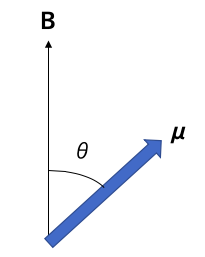
\includegraphics{./images/磁気モーメント.png}
\caption{磁気モーメント}
\end{figure}

\begin{itemize}
\item
  上の図のような磁場\({\bf B}\)中の磁気モーメント\({\bf \mu}\)を考える

  \begin{itemize}
  \tightlist
  \item
    磁気モーメントのエネルギー\({\bf E}\)は、以下のように表される
  \end{itemize}
\end{itemize}

\begin{eqnarray}
E = - \mu\bullet {\bf B}
\end{eqnarray}

\begin{itemize}
\item
  \texttt{磁気モーメント}が磁場方向を向くと最小になる

  \begin{itemize}
  \item
    磁場をかけると、磁気モーメントには\texttt{トルク}が作用する
  \item
    仮に磁気モーメントが全く角運動量を伴わないとすると、トルクによって磁気モーメントは磁場方向に傾くはずである
  \end{itemize}
\end{itemize}

\begin{eqnarray}
{\bf G} = - \mu\times {\bf B}
\end{eqnarray}

    \begin{itemize}
\item
  ただし、\texttt{磁気モーメント}は角運動量\({\bf L}\)を伴い、トルクは角運動量の変化率に等しいので、以下の式で表される

  \begin{itemize}
  \item
    \$ \{\bf \mu\}\(の経時変化が\)\{\bf \mu\}\(と\)
    \{\bf B\}\$の両方に垂直であることを意味する
  \item
    すなわち、磁場は\$ \{\bf \mu\}\(を\)
    \{\bf B\}\(の方向に傾けるのではなく、\)
    \{\bf B\}\$の周りに回転(\texttt{歳差運動})させる
  \item
    以下の式から、\(| {\bf \mu}|\)が時間変化しないことがわかる
  \item
    これは、ジャイロスコープまたはコマの回転と全く同じである
  \end{itemize}
\end{itemize}

\begin{eqnarray}
\frac{d{\bf \mu}}{dt} = \gamma {\bf \mu}\times {\bf B}
\end{eqnarray}

    \subsubsection{ラーモア歳差運動}\label{ux30e9ux30fcux30e2ux30a2ux6b73ux5deeux904bux52d5}

\begin{itemize}
\item
  \$ \{\bf B\}\(がz方向で、\) \{\bf \mu\}\(は最初\)xz\(面内にあり、\)
  \{\bf B\}\(と角度\)\theta\$をなすとする

  \begin{itemize}
  \tightlist
  \item
    この時、以下の式が成立する
  \end{itemize}
\end{itemize}

\begin{eqnarray}
\frac{d{\bf \mu_x}}{dt} = - \gamma B\mu_y\\
\frac{d{\bf \mu_y}}{dt} = - \gamma B\mu_x\\
\frac{d{\bf \mu_z}}{dt} = 0
\end{eqnarray}

    \begin{itemize}
\item
  \({\bf \mu_z}\)は時間変化しない
\item
  \({\bf \mu_x}\)と\({\bf \mu_y}\)はどちらも振動する

  \begin{itemize}
  \item
    これらの微分方程式の解は、以下の値で得られる
  \item
    \(\omega_L\):\texttt{ラーモア周波数}
  \end{itemize}
\end{itemize}

\begin{eqnarray}
\mu_x(t) = |\mu| \sin \theta \cos(\omega_L t)\\
\mu_y(t) = |\mu| \sin \theta \sin(\omega_L t)\\
\mu_z(t) = |\mu| \cos \theta
\end{eqnarray}

\begin{eqnarray}
\omega_L = \gamma B
\end{eqnarray}

    \begin{itemize}
\item
  磁気回転比\(\gamma\)は比例定数であり、\texttt{角運動量}と\texttt{磁気モーメント}を結びつけると同時に、\texttt{磁場}と\texttt{歳差運動}の周波数を結びつける

  \begin{itemize}
  \item
    この歳差運動現象は、今後取り扱う現象が単純出ないことを暗示している
  \item
    すなわち、磁場は磁気モーメントを揃えるだけでなく、様々な動的効果を誘起する
  \end{itemize}
\end{itemize}

    \subsection{3. ボーア磁子}\label{ux30dcux30fcux30a2ux78c1ux5b50}

\begin{itemize}
\item
  \texttt{原子磁気モーメント}の大きさ、\texttt{磁気回転比}の大きさを求める

  \begin{itemize}
  \tightlist
  \item
    水素原子核を回る1つの電子(電荷:\(-e\)、質量:\(m_e\))
  \end{itemize}
\end{itemize}

\begin{figure}
\centering
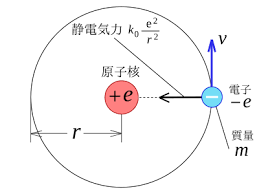
\includegraphics{./images/水素原子.png}
\caption{水素原子}
\end{figure}

\begin{itemize}
\item
  原子の\texttt{周回電流}は、以下の式で表される

  \begin{itemize}
  \item
    回転周期:\(\tau = 2\pi r/ v\)
  \item
    速さ:\(v = |{\bf v}|\)
  \item
    円軌道の半径:\(r\)
  \end{itemize}
\end{itemize}

\begin{eqnarray}
I = - \frac{e}{\tau}
\end{eqnarray}

    \begin{itemize}
\item
  電子の角運動量の大きさ:\(m_e v r\)(基底状態:\(\hbar\))

  \begin{itemize}
  \tightlist
  \item
    電子の\texttt{磁気モーメント}は、以下の式で表される
  \end{itemize}
\end{itemize}

\begin{eqnarray}
\mu = \pi r^2 I = - \frac{e \hbar}{2 m_e}
\end{eqnarray}

    \begin{itemize}
\item
  ここで、\(\mu_b\)を、\texttt{ボーア磁子}として定義する

  \begin{itemize}
  \item
    \texttt{原子磁気モーメント}の大きさを表す単位として用いられる
  \item
    値は、\(9.274 \times 10^{-24} A m^2\)
  \item
    \texttt{磁気モーメント}の符号は、\texttt{負}である(電子の電荷が\texttt{負}であ理、その磁気モーメントは角運動量に反平行であるため)
  \end{itemize}
\end{itemize}

\begin{eqnarray}
\mu_B = - \frac{e \hbar}{2 m_e}
\end{eqnarray}

\begin{itemize}
\tightlist
\item
  電子の\texttt{磁気回転比}は\(\gamma = - frac{e}{2 m_e}\)であるため、\texttt{ラーモア周波数}は以下の式で表される
\end{itemize}

\begin{eqnarray}
\omega_L = |\gamma| B = \frac{e B}{2 m_e}
\end{eqnarray}

    \subsection{4. 磁化と磁場}\label{ux78c1ux5316ux3068ux78c1ux5834}

\begin{itemize}
\item
  \texttt{磁性体}は、\texttt{磁気モーメント}を持つ多数の原子から構成される

  \begin{itemize}
  \item
    \texttt{磁化}\(M\):単位体積当たりの\texttt{磁気モーメント}

    \begin{itemize}
    \item
      通常、このベクトル量は\textbf{連続体近似}で扱われる
    \item
      すなわち、個々の\texttt{原子磁気モーメント}がバラバラに見えない程度に大きなスケールで考える
    \item
      このとき、\(M\)は磁性体の端を除いたあらゆる場所で連続でなめらかなベクトル場と見なされる
    \end{itemize}
  \end{itemize}
\end{itemize}

    \begin{itemize}
\item
  自由空間(真空)には、\texttt{磁化}が存在しない

  \begin{itemize}
  \item
    この時、\texttt{磁場}はベクトル場\(B\)(または\(H\))で、以下の関係式で表される
  \item
    \(B\):\texttt{磁束密度}(単位:\(T\))
  \item
    \(H\):\texttt{磁場の強さ}(単位:\(Am^{-1}\))
  \item
    \(\mu_0 = 4 \pi \times 10^{-7} H m^{-1}\)
  \end{itemize}
\end{itemize}

\begin{eqnarray}
B = \mu_0 H
\end{eqnarray}

    \begin{itemize}
\item
  \texttt{磁性体}内部では、\(B\)と\(H\)の関係は多少複雑になり、2つのベクトル場は大きさと方向が全く異なることもある

  \begin{itemize}
  \tightlist
  \item
    一般的には、これらベクトル間に以下の式が成立する
  \end{itemize}
\end{itemize}

\begin{eqnarray}
B = \mu_0 (H + M)
\end{eqnarray}

    \begin{itemize}
\item
  特に、磁化\(M\)が磁場\(H\)に比例する場合は、その磁性体を\texttt{線形物質}と呼ぶ

  \begin{itemize}
  \item
    この磁性体は、以下の式で表される
  \item
    \(\chi\):\texttt{磁化率}(無次元量)
  \end{itemize}
\end{itemize}

\begin{eqnarray}
M = \chi H
\end{eqnarray}

\begin{itemize}
\item
  この特別な関係が成り立つ場合にも、\(B\)と\(H\)の間には比例関係が存在し、以下の式で表される

  \begin{itemize}
  \tightlist
  \item
    \texttt{比透磁率}:\(\mu_r = 1 + \chi\)(物質ごとに異なる)
  \end{itemize}
\end{itemize}

\begin{eqnarray}
B = \mu_0(1 + \chi)H = \mu_0 \mu_r H
\end{eqnarray}

    \begin{itemize}
\item
  実際は、磁化された媒質中の磁場を定義する際には、注意が必要である

  \begin{itemize}
  \item
    真空に磁場\(B_a\)(あるいは\(H_a\))
  \item
    真空の領域に磁性体を挿入した時に、磁場\(B_i\)(あるいは\(H_i\))は、\(B_a\)(あるいは\(H_a\))と大幅に異なる
  \item
    この差の原因は、磁性体内の磁気モーメント自身が原因となる
  \end{itemize}
\end{itemize}

    \begin{itemize}
\item
  一般には、\(B_i\)と\(H_i\)の値はどちらも測定場所に依存する

  \begin{itemize}
  \tightlist
  \item
    試料を磁化すると、試料内部の磁場同様、試料外部の磁場も影響を受ける
  \end{itemize}
\item
  試料の形状が\textbf{回転楕円体形}の時は例外である

  \begin{itemize}
  \item
    \(a\)、\(b\)、\(c\)は主軸、球(\(a=b=c\))と平面(\(a, b\rightarrow\infty, c=0\))
  \item
    主軸の1つの方向に磁場をかけた時は、試料のあらゆる場所で以下の式が成立する
  \item
    \(N\):反磁場係数(それぞれの場合に応じて適切に取っている)

    \begin{itemize}
    \item
      \(H_i\)を求めるには、\(H_a\)に補正項\(H_d = - N M\)を加える必要がある
    \item
      この補正項を、\texttt{反磁場}と呼ぶ
    \end{itemize}
  \end{itemize}
\end{itemize}

\begin{eqnarray}
H_i = H_a - NM
\end{eqnarray}

\begin{eqnarray}
B_i = \mu_0(H_i + M) = B_a + \mu_0(1 - N)M
\end{eqnarray}

\begin{figure}
\centering
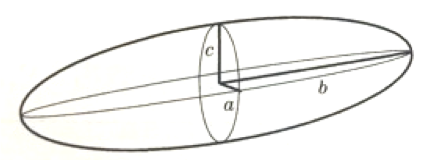
\includegraphics{./images/回転楕円体.png}
\caption{回転楕円体}
\end{figure}

    例)球形試料

\begin{eqnarray}
N = \frac{1}{3}
\end{eqnarray}

球内部の磁場は、以下の式で表される

\begin{eqnarray}
H_i = H_a - \frac{M}{3}
\end{eqnarray}

\begin{eqnarray}
B_i = B_a + \frac{2 \mu_0 M}{3}
\end{eqnarray}

    \begin{itemize}
\item
  \texttt{磁化}が外から加えられた\texttt{磁場}\(|H_a| = \frac{|B_a|}{\mu_0}\)(試料挿入前の値)に比べて大きい時は、\texttt{反磁場補正}を考える必要がある

  \begin{itemize}
  \item
    磁性が弱い場合に限って、このような煩雑さは事実上回避できる
  \item
    \$ \chi \ll 1\$の線形物質では、

    \begin{itemize}
    \item
      \(M \ll H\)
    \item
      \(H_i \approx H_a\)
    \item
      \(B_i \approx \mu_0 H_i\)
    \end{itemize}
  \end{itemize}

  である

  \begin{itemize}
  \item
    つまり、物質中の磁場は外からかけた磁場に等しいと見なして良い
  \item
    反磁場の比較的弱い効果を扱う際には、この近似を用いる
  \item
    強磁性体では反磁場の効果は常に重要である
  \end{itemize}
\end{itemize}

    例)物質固有の磁化率

\begin{eqnarray}
\chi_{固有} = \frac{M}{H_i}
\end{eqnarray}

\begin{itemize}
\item
  実験で測定される量はこの物質固有量ではない

  * 磁化\(M\)は外から加える磁場\(H_a\)に対する応答として観測されるため

  \begin{itemize}
  \tightlist
  \item
    測定値は、以下の式で表される
  \end{itemize}
\end{itemize}

\begin{eqnarray}
\chi_{実験} = \frac{M}{H_a}
\end{eqnarray}

\begin{itemize}
\tightlist
\item
  これらの2つの物質量の間には、以下の関係がある
\end{itemize}

\begin{eqnarray}
\chi_{実験} = \frac{M}{H_i + NM} = \frac{\frac{M}{H_i}}{1+\frac{NM}{H_i}} = \frac{\chi_{固有}}{1 + N \chi_{固有}}
\end{eqnarray}

\begin{itemize}
\item
  \(\chi \ll 1\)の時は、\(\chi_{固有}\)と\(\chi_{実験}\)の差は取るに足らない
\item
  \(\chi_{固有}\)が1に近いか、あるいは1より大きい場合、差は大きくなる

  \begin{itemize}
  \tightlist
  \item
    例)強磁性体が高温側からキュリー温度に近づく時は、\$\chi\emph{\{固有\}
    \rightarrow\infty \(であるが、\)\chi}\{実験\}
    \rightarrow \frac{1}{N}\$
  \end{itemize}
\end{itemize}

    \begin{itemize}
\item
  強磁性体材料は試料全体で磁気モーメントを持たないことがある

  \begin{itemize}
  \item
    強磁性体には\texttt{磁区}が存在しているため
  \item
    それぞれの\texttt{磁区}は一様であるが、\texttt{磁化}の方向は隣接する\texttt{磁区}とは異なる
  \item
    微視的なスケールで全ての\texttt{磁気モーメント}が局所的に存在していても、試料に\texttt{磁化}が現れないことがある
  \end{itemize}
\end{itemize}

    \begin{longtable}[]{@{}ll@{}}
\toprule
版 & 年/月/日\tabularnewline
\midrule
\endhead
初版 & 2019/03/01\tabularnewline
\bottomrule
\end{longtable}


    % Add a bibliography block to the postdoc
    
    
    
    \end{document}
